\documentclass{article}
\usepackage{notes}

\newcommand{\solution}{\textbf{Solution: }}
\newcommand{\Var}{\text{Var}}
\newcommand{\Cov}{\text{Cov}}

\title{CS189, HW5: Decision Trees}

\begin{document}

\maketitle

\noindent In this homework, you will implement decision trees and random forests for classification on 3 datasets: 1) the spam dataset, 2) a census income dataset to predict whether or not a person makes over 50k in income, and 3) a Titanic dataset to predict Titanic survivors. The data is available on Piazza. \\

\noindent In lectures, you were given a basic introduction to decision trees and how such trees are trained. You were also introduced to random forests. Feel free to research different decision tree techniques online. You do not have to implement boosting, though it might help with Kaggle.

\begin{enumerate}
    \item Implement decision trees. See the Appendix for more information. You are not allowed to use any off-the-shelf decision tree implementation. Some of the datasets are not “cleaned,” i.e. there are missing values, so you can use external libraries for data preprocessing (in fact, we recommend it). Be aware that some of the later questions might require special functionality that you need to implement (e.g. max depth stopping criteria, visualizing the tree, tracing the path of a sample through the tree). You can use any programming language you wish as long as we can read and run your code with minimal effort. In this part of your writeup, \textbf{include your decision tree code.}
    \begin{mdframed}
    (See attached code)
    \end{mdframed}

    \item Implement random forests. You are not allowed to use any off-the-shelf random forest implementation. If you architected your code well, this part should be a (relatively) easy encapsulation of the previous part. In this part of your writeup, \textbf{include your random forest code.}
    \begin{mdframed}
    (See attached code)
    \end{mdframed}

\newpage
    \item Describe implementation details. We aren’t looking for an essay; 1-2 sentences per question is enough.
    \begin{enumerate}
        \item How did you deal with categorical features and missing values?
        \begin{mdframed}
          \begin{itemize}
          \item \textbf{categorical features}: I used
            \texttt{DataFrame.get\_dummies()} from \texttt{pandas} to one-hot
            encode categorical features.
          \item \textbf{Missing values}: Quick rough treatment only so far: I
            removed any row that had a missing value in a column, when that
            column had fewer than 5 missing values. I dropped any remaining
            columns that had missing data.
          \end{itemize}
        \end{mdframed}

        \item What was your stopping criterion?
        \begin{mdframed}
          The code has a \texttt{max\_depth} parameter. Setting it to infinity
          does not stop early.
        \end{mdframed}

        \item Did do anything special to speed up training?
        \begin{mdframed}
          I used the splitting algorithm outlined in lectures.

          I used \texttt{multiprocessing} to compute some accuracies in parallel.
        \end{mdframed}

        \item How did you implement random forests?
        \begin{mdframed}
          I changed my \texttt{DecisionTree} class to accept three additional parameters:
          \texttt{n\_trees}, \texttt{randomize\_features}, \texttt{randomize\_observations}.
        \end{mdframed}

        \item Anything else cool you implemented?
        \begin{mdframed}
          The \texttt{model\_selection.get\_error\_rates()} function was useful
          for running error rate experiments (varying models and data).
        \end{mdframed}
    \end{enumerate}

\newpage
  \item Performance evaluation. For each of the 3 datasets, train a decision
    tree and random forest and report your training and validation
    accuracies. You should be reporting 12 numbers (3 datasets $\times$ 2
    classifiers $\times$ 2 data splits). In addition, for each of the 3
    datasets, train your best model and submit your predictions to
    Kaggle. Include your Kaggle display name and your public scores on each
    dataset. You should be reporting 3 numbers.
    \begin{mdframed}
      \begin{tabular}{l|l|l|l|l|l|l}
                              & spam     & spam (RF) & census & census (RF) & titanic & titanic (RF) \\
        \hline
        max depth             & $\infty$ & $\infty$  & 6      & 6           & 2       & 2           \\
        num trees             &          & 10        &        & 10          &         & 10          \\
        training accuracy     & .852     & .528      & .840   & .553        & .813    & .449        \\
        validation accuracy   & .795     & .530      & .834   & .554        & .797    & .476        \\
        kaggle accuracy       & .809     &           & .837   &             & .826    &             \\
      \end{tabular}

    \end{mdframed}

\newpage
    \item Writeup requirements for the spam dataset:
    \begin{enumerate}
        \item If you use any other features or feature transformations, explain what you did in your report. You may choose to use something like bag-of-words. You can implement any custom feature extraction code in \texttt{featurize.py}, which will save your features to a \texttt{.mat} file.
        \begin{mdframed}
          No extra features.
        \end{mdframed}

      \item For your decision tree, and for a data point of your choosing from
        each class (spam and ham), state the splits (i.e. which feature and
        which value of that feature to split on) your decision tree made to
        classify it.


        \begin{mdframed}
        $y = 0$:
        \begin{verbatim}
        feature 28 <= 0.00
        feature 29 <= 0.00
        feature 7 <= 0.00
        feature 19 <= 0.00
        feature 25 <= 1.00
        feature 13 <= 0.00
        feature 3 <= 0.00
        feature 0 <= 0.00
        feature 26 <= 0.00
        feature 31 <= 0.00
        feature 6 <= 0.00
        feature 16 <= 0.00
        feature 20 <= 0.00
        feature 30 <= 0.00
        feature 1 <= 0.00
        feature 5 <= 0.00
        feature 14 <= 0.00
        feature 21 <= 0.00
        feature 17 <= 0.00
        feature 2 <= 1.00
        feature 4 <= 0.00
        feature 18 <= 0.00
        feature 24 <= 0.00
        feature 10 <= 0.00
        feature 27 <= 1.00
        feature 15 <= 2.00
        feature 27 <= 0.00
        feature 12 <= 1.00
        feature 12 <= 0.00
        feature 8 <= 0.00
        feature 15 <= 0.00
        feature 2 <= 0.00
        feature 23 <= 0.00
        feature 25 <= 0.00
        feature 22 <= 0.00
        Classified as 0.0
        \end{verbatim}
        \end{mdframed}

        \begin{mdframed}
        $y=1$:
        \begin{verbatim}
        feature 28 <= 0.00
        feature 29 <= 0.00
        feature 7 <= 0.00
        feature 19 <= 0.00
        feature 25 <= 1.00
        feature 13 <= 0.00
        feature 3 <= 0.00
        feature 0 <= 0.00
        feature 26 <= 0.00
        feature 31 <= 0.00
        feature 6 <= 0.00
        feature 16 <= 0.00
        feature 20 <= 0.00
        feature 30 <= 0.00
        feature 1 <= 0.00
        feature 5 <= 0.00
        feature 14 <= 0.00
        feature 21 <= 0.00
        feature 17 <= 0.00
        feature 2 <= 1.00
        feature 4 <= 0.00
        feature 18 <= 0.00
        feature 24 <= 0.00
        feature 10 <= 0.00
        feature 27 <= 1.00
        feature 15 <= 2.00
        feature 27 > 0.00
        feature 2 <= 0.00
        feature 15 > 0.00
        Classified as 0.0
        \end{verbatim}
        \end{mdframed}

      \item For random forests, find and state the most common splits made at
        the root node of the trees.
        \begin{mdframed}
        \begin{verbatim}
        feature 1 > 0.00                                   (9 trees)
        feature 4 > 0.00                                   (7 trees)
        feature 3 > 0.00                                   (5 trees)
        feature 2 > 0.00                                   (4 trees)
        feature 0 > 0.00                                   (4 trees)
        feature 1 > 3.00                                   (1 trees)
        \end{verbatim}
        \end{mdframed}
    \end{enumerate}

\newpage
    \item Writeup requirements for the census dataset:
    \begin{enumerate}
        \item Do 4a, but for the census dataset
        \begin{mdframed}
          No extra features.
        \end{mdframed}

        \item Do 4b, but for the census dataset
        \begin{mdframed}

$y=0$:
\begin{verbatim}
capital-gain <= 6849.00
age > 27.00
education-num <= 12.00
White <= 0.00
education-num <= 8.00
hours-per-week > 42.00
age > 57.00
Classified as 0
\end{verbatim}

$y=1$:
\begin{verbatim}
capital-gain > 6849.00
education-num <= 9.00
capital-gain <= 20051.00
age <= 61.00
hours-per-week <= 35.00
age > 34.00
Classified as 1
\end{verbatim}

        \end{mdframed}

        \item Do 4c, but for the census dataset
        \begin{mdframed}
\begin{verbatim}
age > 27.00                                        (6 trees)
education-num > 6849.00                            (3 trees)
fnlwgt > 0.00                                      (3 trees)
age > 0.00                                         (3 trees)
age > 12.00                                        (3 trees)
education-num > 27.00                              (3 trees)
age > 6849.00                                      (2 trees)
fnlwgt > 12.00                                     (2 trees)
fnlwgt > 41.00                                     (1 trees)
fnlwgt > 6849.00                                   (1 trees)
fnlwgt > 27.00                                     (1 trees)
age > 1844.00                                      (1 trees)
age > 41.00                                        (1 trees)
\end{verbatim}
        \end{mdframed}

      \item Generate a random 80/20 training/validation split. Train decision
        trees with varying maximum depths (try going from depth = 1 to depth =
        40) with all other hyperparameters fixed. Plot your validation
        accuracies. Which depth had the highest validation accuracy? Write 1-2
        sentences explaining the behavior you observe in your plot. If you find
        that you need to plot more depths, feel free to do so.
        \begin{mdframed}
          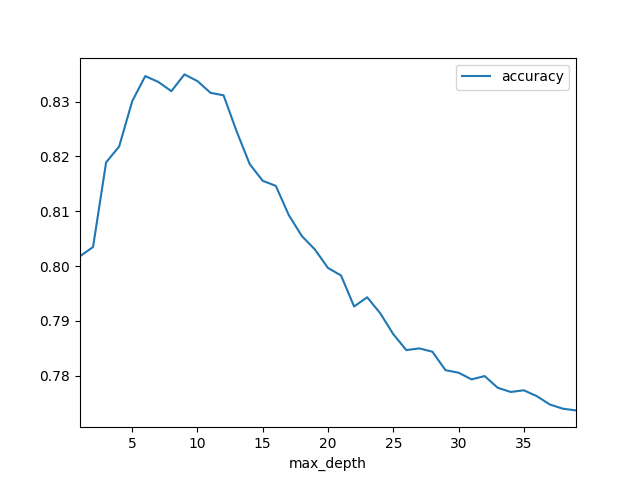
\includegraphics[width=400pt]{img/census_depth_experiment.png}

          Trees with depth around 6 had the highest validation accuracy.\\

          At depths less than 6, the variance of the classifier is low but the
          bias of the classifier is too high (underfits the training data).\\

          At depths greater than 6, the bias of the classifier is low but the
          variance of the classifier is too high (overfits the training data).
        \end{mdframed}

    \end{enumerate}

\newpage
    \item Writeup requirements for the Titanic dataset:
    \begin{enumerate}
    \item Train a very shallow decision tree (for example, a depth 3 tree,
      although you may choose any depth that looks good) and visualize your
      tree. Include for each non-leaf node the feature name and the split rule,
      and include for leaf nodes the class your decision tree would assign.
        \begin{mdframed}
          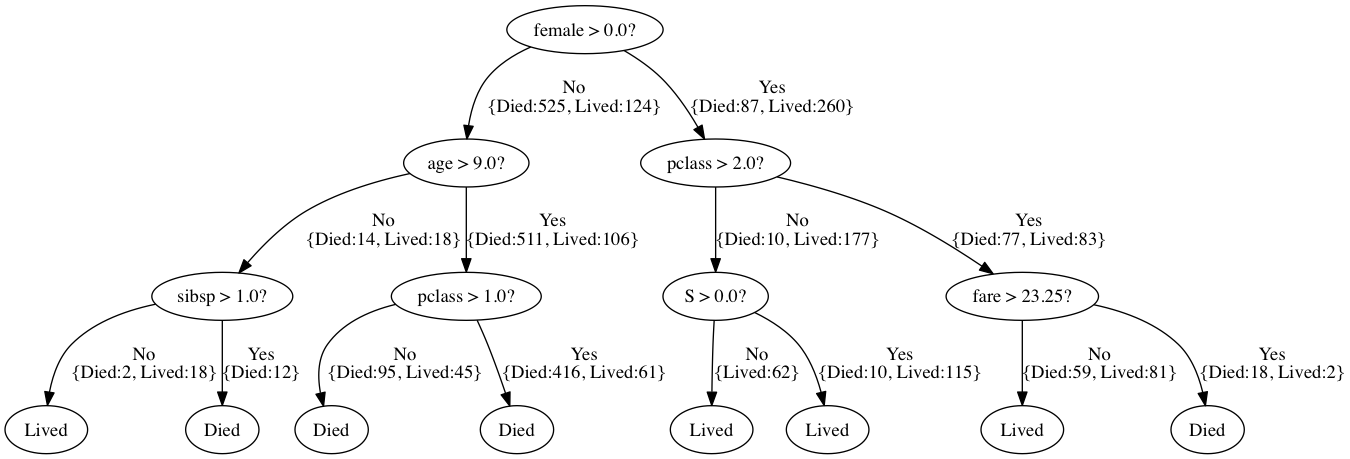
\includegraphics[width=400pt]{img/titanic.png}
        \end{mdframed}
    \end{enumerate}
\end{enumerate}


\end{document}
